\section{Durchführung}
\label{sec:Durchführung}

\subsection{Versuchsaufbau}
Das Licht der Rubidium-Spektrallampe trifft zunächst auf eine Sammellinse. Anschließend geht es durch einen Interferenzfilter (D$_1-$Filter), der nur Licht mit einer Wellenlänge von $\lambda = \SI{794.8}{\nano\meter}$ durchlässt. Der darauffolgende Polarisationsfilter und die $\lambda / 4-$Platte bewirken, dass das austretende Licht zirkular-polarisiert ist (rechtszirkular?). Dieses Licht trifft auf die von drei Helmholtz-Spulenpaaren umgebene Dampfzelle. Das transmittierte Licht wird mithilfe einer Sammellinse auf einen Lichtdetektor fokussiert, welcher an einem Oszilloskop angeschlossen ist. \cite{V21}
Dieser Versuchsaufbau ist in Abb. \ref{fig:aufbau} zu sehen.

\begin{figure}
    \centering
    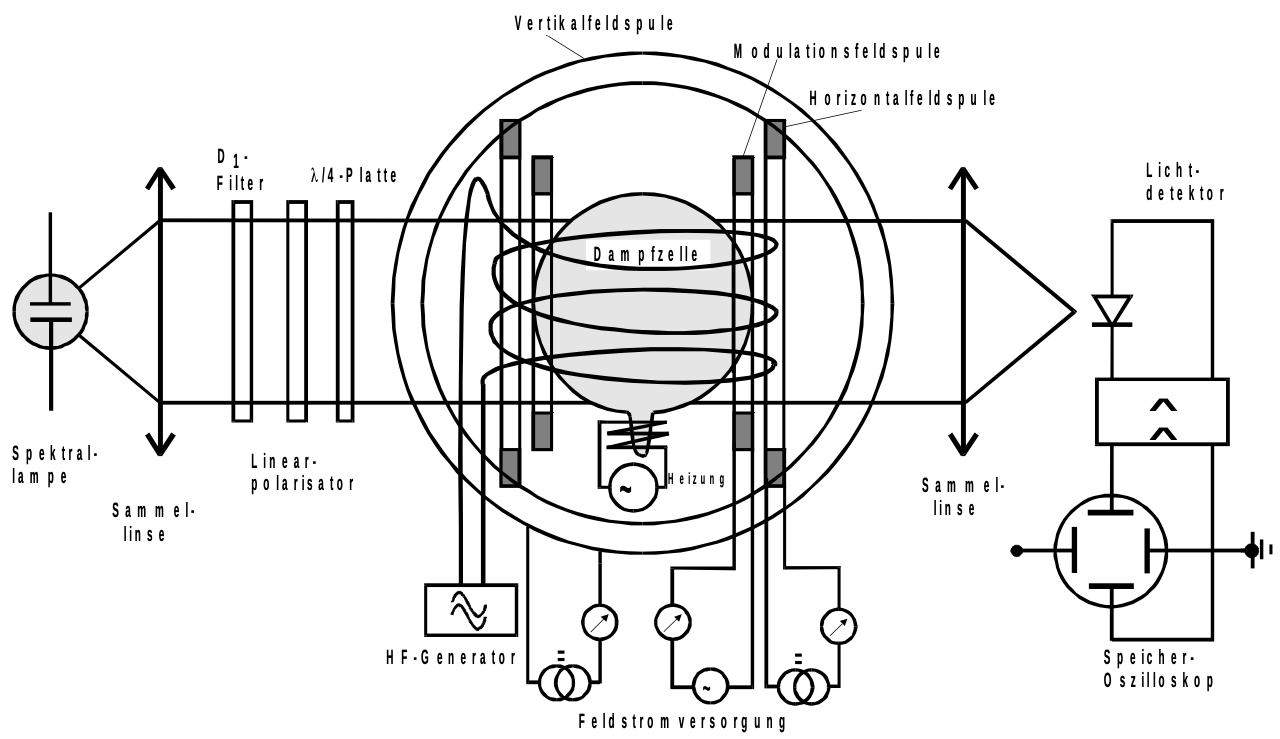
\includegraphics[width=15cm]{fotos/aufbau.png}
    \caption{Der Aufbau der Messapparatur. \cite{V21}}
    \label{fig:aufbau}
\end{figure}

\subsection{Justierung/ vor Beginn des Versuchs}
Der Ofen, der die Dampfzelle heizt, wird eine halbe Stunde vor Beginn eingeschaltet. \cite{V21}

Zunächst wird der Strahlengang so justiert, dass die Intensität maximal ist. Diese wird am Lichtdetektor gemessen.
%Dazu ist der "Gain" überall $\num{1}$ und die Zeitkonstante beträgt $\SI{100}{\milli\second}$.
Anschließend werden die beiden Linsen eingesetzt und mithilfe der Signalstärke am Galvanometer justiert.
Nachdem weitere optische Elemente eingesetzt sind, wird der ganze Aufbau mit einer schwarzen Decke abgedeckt. \cite{V21}

Vor der Messung muss das Erdmagnetfeld kompensiert werden.
Dazu wird durch einen Stromfluss durch die Sweep-Spule (Modulationsfeldspule) die horizontale Magnetfeldkomponente auf Null reguliert. Anschließend wird mithilfe der Vertikalfeldspule ein schmaler Peak eingestellt, um die Vertikalkomponente des Erdmagnetfeldes zu kompensieren. Die Messapparatur wird so ausgerichtet, dass der Lichtstrahl in Nord-Süd-Richtung verläuft. \cite{V21}

Die Eigenschaften der Spulen sind in Tab. \ref{tab:spule} aufgelistet. 
Alle drei Spulen sind Helmholtzspulen-Paare. Für sie gilt, dass die Magnetfeldstärke 
\begin{equation*}
    B = \mu_0 \cdot \frac{8 \cdot I \cdot N}{\sqrt{125} R}
\end{equation*}
beträgt mit der Stromstärke $I$, der Windungszahl $N$ und dem Radius $R$. 

\begin{table}\caption{Die TEM$_{00}$-Mode. Der Abstand senkrecht zur Laserachse ist gegen die Stromstärke aufgelistet.}
    \label{tab:mode0}
    \centering
    \sisetup{round-mode = places, round-precision=1, round-integer-to-decimal=true}
    \begin{tabular}{c | S[] S[] S[]} 
    \toprule
    {Spule} & {$R / \si{\centi\metre}$} & {$R$} & {Verstärkung} \\
    \midrule
    Horizontal & 15.79 & 154 & 0.3 \\
    Sweep & 16.39 & 11 & 0.1 \\ 
    Vertikal & 11.735 & 20 & 0.1 \\ 
    \bottomrule
\end{tabular}\end{table}

\subsection{Resonanzstelle}
Die Frequenzen (der Sinusspannung) an der RF-Spule (Sweep-Spule und horizontale Spule) werden zwischen $\SI{100}{\kilo\hertz}$ und $\SI{1}{\mega\hertz}$ in $\SI{100}{\kilo\hertz}$ Schritten variiert. Dabei wird die Stärke des gesamten Horizontalfeldes in Abhängigkeit von der Resonanzfrequenz für beide Rb-Isotope (bei induzierter Emission) gemessen. Die Resonanzen für beide Isotope sollen sichtbar gemacht werden. Bei Frequenzen höher  ca. $\SI{200}{\kilo\hertz}$ wird zusätzlich ein horizontales Feld angelegt (Sweep-Spule reicht nicht mehr aus).

%daraus Horizontalkomponente des lokalen Erdmagnetfeldes und Landé-Faktoren der beiden Isotope
%-> aus Landé-Faktoren die Kernspins ermitteln

Es wird ein Foto eines typischen Signalbildes (bei $\SI{100}{\kilo\hertz}$) gemacht. %richtig?

%bei 100kHz: Isotopenverhältnis aus den beobachteten Amplituden ermitteln
%von der Natur gegebenes Verhältnis?

%Größe des quadratischen Zeeman-Effekts abschätzen

Die Frequenz wird auf $\SI{100}{\kilo\hertz}$ und das Magnetfeld auf die Resonanzstelle von einem Rb-Isotop gestellt. Ein zweiter Funktionsgenerator erzeugt eine Rechteckspannung. %und was macht man damit?
Die Kurve wird aufgenommen. %und mit e-Fkt fitten

Die Perioden der Oszillationen werden als Funktion der RF-Amplituden bestimmt. Dazu wird am Funktionsgenerator eine Frequenz von $\SI{100}{\kilo\hertz}$ eingestellt und die Spannung wird von $\SI{0.5}{\volt}$ auf $\SI{10}{\volt}$ in $\SI{1}{\volt}$ Schritten erhöht.
%für beide Isotope: Periode gegen RF-Amplitude (in V) plotten, mit Hyperbel-Funktion fitten
